\newpage
\section{Data Warehouse[AA]}\label{ssec:dw}
Referenzinformationen für dieses Unterkapitel stammen aus dieser Quelle. (vgl. \cite{ionis_dwh_2020})
\subsection{Definition}
Ein Data Warehouse (DW) ist ein zentrales Datenbanksystem, um Daten effektiv in einem Unternehmen analysieren zu können. Zahlreiche Unternehmen laden ihre historischen Daten in ein Data Warehouse, um jene Daten zu analysieren. Um mit ihnen Prognosen geben zu können, wie das Unternehmen in der Zukunft agieren soll. Im Data Warehousing gibt es zwei Daten, die unterschieden werden müssen(\ref{ssec:Operative-Daten} \& \ref{ssec:Dispositive-Daten}). Außerdem ermöglicht ein Data Warehouse die Aggregation betrieblicher Kennzahlen im Rahmen des OLAP (Online Analytic Processsings).\\
Durch das Sammeln aller relevanten Unternehmensdaten dient das Data Warehouse auch als Wissens Managementsystem. Im Regelfall werden den Anwendern nur der Lesezugriff gewährt, aber keine Schreibrechte, um Daten zu ändern oder gar zu löschen. Ein Data Warehouse ist zudem auch noch Datenbasis für Data Mining Methoden und ist die Grundlage aller Überlegungen im Rahmen des Leistungsmanagements und der strategischen Unternehmensausrichtung.
\subsection{Operative Daten}\label{ssec:Operative-Daten}
Bei diesen Daten handelt es sich um transaktionsorientierte Daten und Informationen, die während des Tagesbetriebs in einem Unternehmen anfallen und von Administrations- und Abrechnungssystemen generiert werden. Zu Datenquellen dieser Daten gehören Buchhaltungsprogramme, Warenwirtschaftssysteme, Enterprise-Ressource-Planung (ERP) oder Auskunft- und Bestellsysteme.
\subsection{Dispositive Daten}\label{ssec:Dispositive-Daten}
Werden operative Daten in ein zentrales System aggregiert, gelagert und für Analysen benutzt und verarbeitet, spricht man von dispositiven Daten.
\newpage
\subsection{Data-Warehouse-Architektur}
Das Beschaffen und die Auswertung der Daten eines Data Warehouses wird Data Warehousing genannt und umfasst drei Phasen.
\begin{itemize}
\item Datenbeschaffung und Datenintegration
\item Datenhaltung
\item Datenauswertung und Datenanalyse
\end{itemize}
Diese Phasen spiegeln sich in der Referenzarchitektur von Data Warehouse Systemen wider. Natürlich unterscheidet sich die Systemarchitektur eines Data Warehouses je nach Produkt und Anbieter, jedoch orientiert sich der technische Aufbau an einem Muster, das sich erneut in drei Ebenen gliedern lässt.
\begin{itemize}
\item Datenerfassungsebene
\item Datenhaltungsebene
\item Datenbereitstellungsebene
\end{itemize}
Es gibt auch eine zentrale Kontrollkomponente. Dies ist der Data Warehouse Manager, der jeder Ebene spezielle Administrationsfunktionen zuordnet. Die einzelnen Komponenten eines Data Warehouses müssen nicht von einem einzigen Anbieter stammen, denn jeweilige Services können von unterschiedlichen Softwareprodukten oder Individuallösungen bereitgestellt werden.
In dieser Graphik wird das gesamte Referenzmodell eines Data Warehouses bildlich dargestellt.
\begin{figure}[H]
\centering
  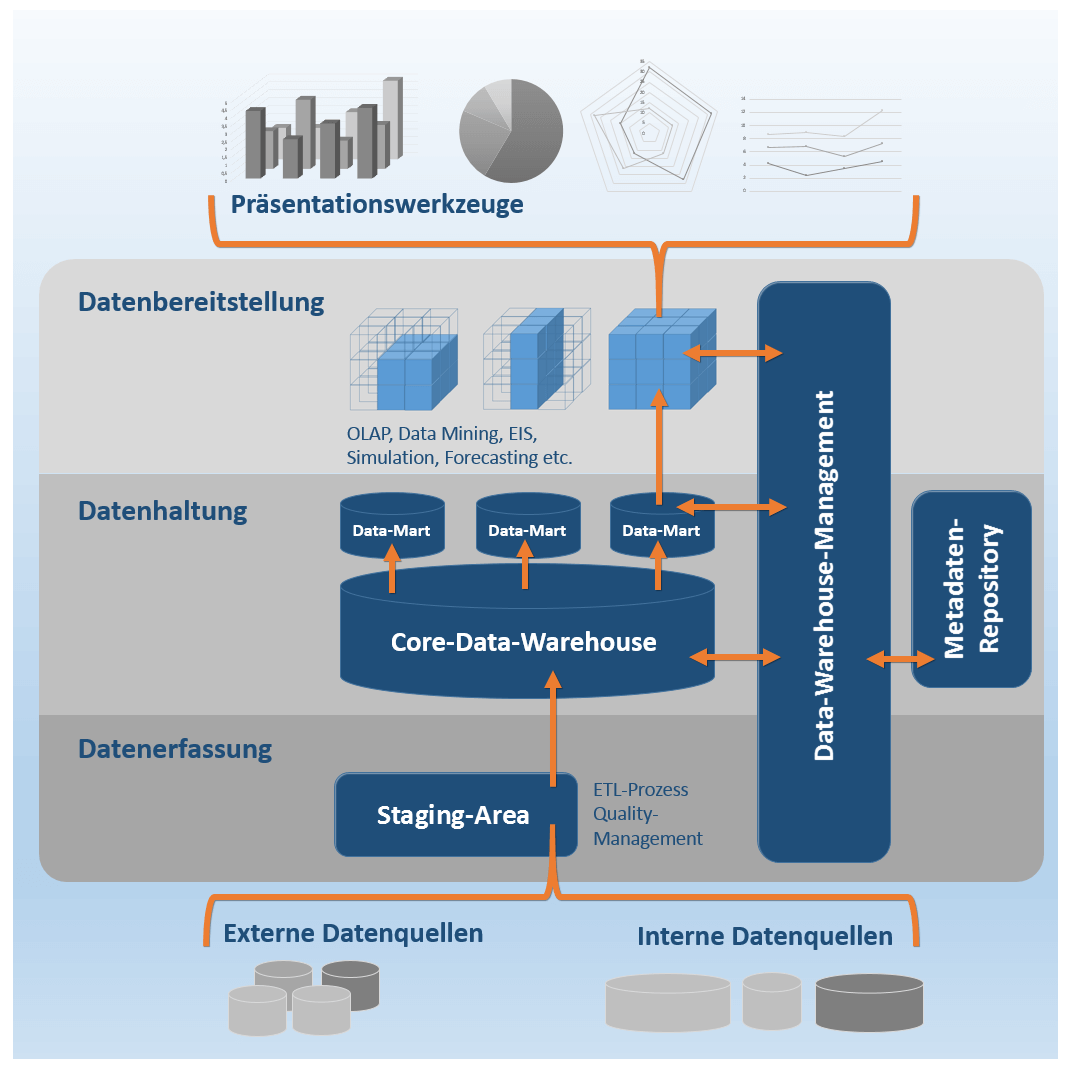
\includegraphics[scale=0.4]{images/data-warehouse-referenzarchitektur.png}
  \caption[DWH Referenzarchitektur (01.04.2020)]{DWH Referenzarchitektur (01.04.2020)}
  \url{https://www.ionos.at/digitalguide/fileadmin/DigitalGuide/Screenshots/data-warehouse-referenzarchitektur.png}
  \label{fig:DWH-RA}
\end{figure}
\newpage
\subsection{Datenerfassungsebene}
Bevor das Data Warehouse Daten bekommen kann, müssen diese oft sehr heterogenen Daten in eine einheitliche Form transformiert werden. Ein Data Warehouse bekommt Daten sowohl aus internen (\ref{ssec:Interne-Daten}) als auch aus externen (\ref{ssec:Externe-Daten}) Datenquellen. Systeme in dieser Ebene stellen Schnittstellen zu operativen Systemen eines Unternehmens bereit und kommen in der ersten Phase des Data Warehousings zum Einsatz. Zentrale Funktionen dieser Phase sind die Datenbeschaffung und Datenintegration. Diese Ebene eines Data Warehouses kann auch eine Staging Area(\ref{ssec:Staging-Area}) beinhalten. Da unterschiedlichste Daten von verschiedensten Quellen in ein DW zusammengefügt werden, muss sich die Datenintegration auf diverse Werkzeuge verlassen, die eine Transformation und Bereinigung der Daten ermöglichen. Diese Werkzeuge können in folgende Kategorien, unterteilt werden (\ref{ssec:Data-Migration} \& \ref{ssec:Data-Scrubbing} \& \ref{ssec:Data-Auditing}). Nach der Datenintegration folgt die Übernahme der Daten in die zentrale Datenbank, in das Core Data Warehouse. Dieser Schritt wird durch Programme unterstützt, die folgende Funktionen bereitstellen.
\begin{itemize}
\item Integritätsbedingungen prüfen
\item Daten sortieren
\item Aggregationen berechnen
\item Zugriffsstrukturen berechnen
\item Daten für einen effizienten Zugriff partitionieren
\end{itemize}
\subsection{Interne Daten}\label{ssec:Interne-Daten}
Interne Daten können von operativen Systemen kommen. Da wären zuallererst, Enterprise Resource Planning-Systeme (ERP) und Customer Relationship Management Systeme(CRM). Auf der anderen Seite können Daten aus operativen Datenbanken bezogen werden. Aus Content Management Systemen(CMS) oder auch aus Flat Files. Beispiele zu diesen wären Excel-, CSV- und Textdateien. Mails und andere Quellen können auch Daten enthalten, die wichtig für ein Data Warehouse sind.
\subsection{Externe Daten}\label{ssec:Externe-Daten}
Dies sind Daten die von externen Dienstleistern stammen. Aus externen Anwendungen und Systemen, wie etwa Websites, Social Media und Cloud Services.
\subsection{Staging Area eines DW}\label{ssec:Staging-Area}
Eine Staging Area ist ein temporärer Bereich der Datenbank, in dem die Vorverarbeitung der zu ladenden Daten stattfindet. Bei mehr komplexen ETL-Prozessen ist so ein Staging erforderlich.
\subsection{ETL für Datawarehouse}\label{ssec:ETL-DW}
Die meisten Data Warehouse stellen im Rahmen der Datenintegration, OLAP-Funktionalitäten zur Verfügung. Diese Funktionalitäten ermöglichen es, Daten in mehrdimensionalen Strukturen darzustellen. Durch den vorher beschriebenen ETL Prozess(\ref{ssec:ETL-DW}) werden Daten aus verschiedensten Quellen extrahiert, danach vorbereitet und anschließend transformiert. Daraufhin werden diese transformierten Daten in das Data Warehouse geladen und dort abgespeichert. Da OLAP eine Analysemethode ist, die der Verdichtung managementrelevanter Unternehmensdaten dient, ist es möglich dieses Verfahren auf den ETL-Prozess zu übertragen.
\subsection{Data Migration Tools}\label{ssec:Data-Migration}
Programme für Datenmigrationen sind dazu da, einfache Transformationsregeln zu definieren und heterogene Ausgangsdaten in ein einheitliches Zielformat zu transformieren.
\subsection{Data Scrubbing Tools}\label{ssec:Data-Scrubbing}
Programme die Data Scrubbing unterstützen, stützen sich auf den Fuzzy Logic Ansatz sowie neuronale Netze. Ziel dieses Ansatzes ist es, die Datenqualität zu verbessern. Dies geschieht indem Fehler, Lücken und Wiederholungen in Datensätzen durch vordefinierten Regeln, Algorithmen oder Lookup Tabels ausgebessert werden. In diesem Fall könnte man auch von Qualitätsmanagement sprechen.
\subsection{Data Auditing Tools}\label{ssec:Data-Auditing}
Dieses Werkzeug kommt zum Einsatz um Regeln und Beziehungen zwischen Daten zu ermitteln. Auch ist es so möglich, Daten zu identifizieren, die gegen die Regeln verstoßen und somit fehlerhaft sind.
\newpage
\subsection{Datenhaltungsebene}
Dies ist die Kernebene des Data Warehouses. In dieser Ebene liegt das Core Data Warehouse. Daten, die extrahiert worden sind, werden in das Data Warehouse meist in mehrdimensionalen Matrizen gespeichert. Doch wird für die Speicherung bestimmte Schemata verwendet. Dies sind das Star-(\ref{ssec:Star-Schema}) oder das Snowflake Schemata(\ref{ssec:Snowflake-Schema}). Diese beinhalten jedoch selten den gesamten Datenbestand des Data Warehouses. Um effiziente Auswertung aus den Daten zu erstellen, werden üblicherweise Datenausschnitte, sogenannte Data Marts(\ref{ssec:Data-Marts}) angelegt.
\subsection{Data Marts}\label{ssec:Data-Marts}
Ein Data Mart ist eine Kopie eines Bestandteils des Data Warehouses. In der Regel sind diese Daten nicht persistent und Data Marts werden oft nur als Zwischenspeicher genutzt. Es gibt jedoch auch unabhängige Data Marts die separate Datenausschnitte dauerhaft lagern und speichern können.
\subsection{Faktentabelle}\label{ssec:Fakten-Tabelle}
Die Faktentabelle beinhaltet verschiedenste Fakten. Diese sind Kennzahlen oder Ergebniszahlen eines Unternehmes, die kontinuierlich in diese Tabelle gespeichert werden.
\subsection{Dimensionstabelle}\label{ssec:Dimensions-Tabelle}
In diesen Tabellen werden Attribute gespeichert, die die Daten der Faktentabelle beschreiben. In einer Dimensionstabelle ist eine Sammlung von Referenzinformationen zu den in der Faktentabelle gespeicherten Ereignissen.
\subsection{3NF}\label{ssec:Dritte-NF}
Alle Data Warehouses können in der dritten Normalform gehalten werden. Doch ist es besser auf andere Schemata auszuweichen, da hier viele Joins getätigt werden müssen um die Daten zu analysieren. Doch hier wird kosteneffizient gespeichert und es kommen keine Redundanzen auf.
\begin{figure}[H]
\centering
  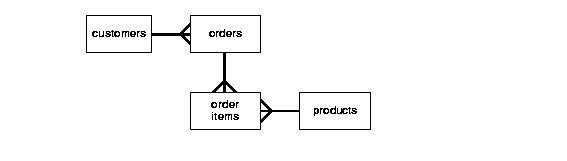
\includegraphics[scale=0.5]{images/3NF.png}
  \caption[3NF (01.04.2020)]{3NF (01.04.2020)}
  \url{https://docs.oracle.com/cd/B10500_01/server.920/a96520/dwhsg108.gif}
  \label{fig:3NF}
\end{figure}
Dieser Auszug wurde durch folgende Quelle inspiriert. \cite{oracle_schema_2020}
\subsection{Star Schema}\label{ssec:Star-Schema}
Bei dem Star Schema handelt es sich um eine Form des Entity Relationship Diagrams oder kurz ERD. Dies ist eine grafische Darstellung der Tabellenstruktur einer Datenbank, bei der die Entitäten sowie die Beziehungen dargestellt werden. Dieses Schema dient der Visualisierung multidimensionaler Datenstrukturen. Jedes Schema besteht aus einer Faktentabelle und mehreren Dimensionstabellen, die sternförmig gruppiert sind. In einem Star Schema ist nur die Faktentabelle mit allen Dimensionstabellen via Fremdschlüssel verbunden. Verbindungen zwischen einzelnen Dimensionstabellen gibt es in diesem Schema nicht.
\begin{figure}[H]
\centering
  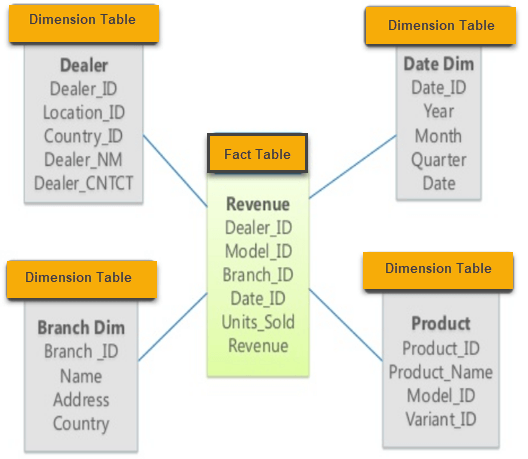
\includegraphics[scale=0.4]{images/Star.png}
  \caption[Star Schema (01.04.2020)]{Star Schema (01.04.2020)}
  \url{https://www.guru99.com/images/1/022218_0758_StarandSnow1.png}
  \label{fig:Star-Schema}
\end{figure}
\newpage
\subsection{Snowflake Schema}\label{ssec:Snowflake-Schema}
Dieses Schema stützt sich im Allgemeinen darauf, dass die Dimensionstabellen normalisiert werden, beziehungsweise Daten nicht mehr redundant in den Dimensionstabellen gespeichert werden. Durch diese Aufteilung der Daten entsteht eine Klassifizierung damit diese hierarchisch gelagert werden. Jene Verzweigung erinnert an eine Schneeflocke. Im Gegensatz zum Star Schema verbraucht das Snowflake Schema viel weniger Speicherplatz. Dies gelingt durch die Aufteilung der Daten auf mehrere Tabellen um so Redundanzen zu vermeiden. Oft werden die Dimensionstabllen noch weiter normalisiert, um bessere Strukturen erreichen zu können. Auf diese Art und Weise wird der Umgang mit Daten erleichtert, da diese, wenn es benötigt wird, nur an einer Stelle angepasst werden müssen. \\
Ein Nachteil ist, dass dadurch nicht nur die Datenstruktur um einiges komplexer wird. Außerdem müssen Tabellen gejoint werden, wenn die Daten benötigt werden. Der Join ist einer der aufwendigsten Datenbankzugriffe die es gibt. In der Praxis wird für die Datenstruktur des Core Data Warehouse oft das Snowflake Schema angewendet, während für einzelne Data Marts das Star Schema benutzt wird.
\begin{figure}[H]
\centering
  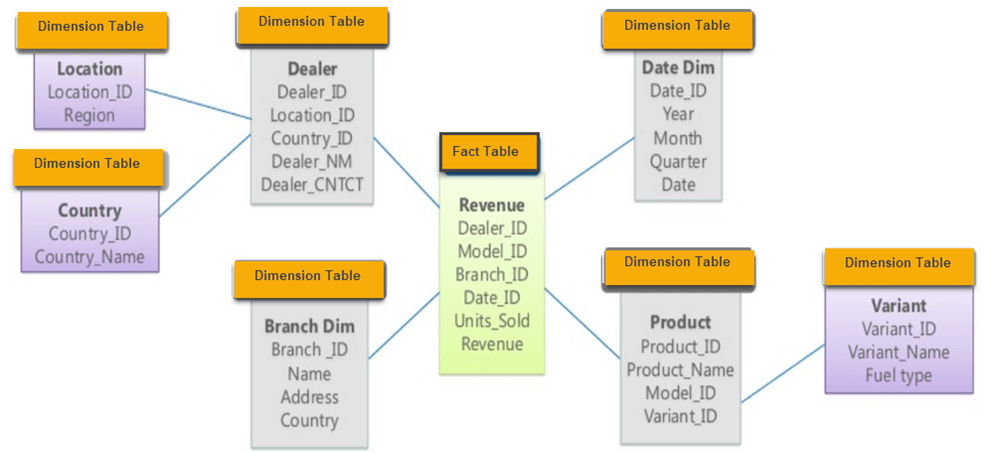
\includegraphics[scale=0.4]{images/Snow.png}
  \caption[Snowflake Schema (01.04.2020)]{Snowflake Schema (01.04.2020)}
  \label{fig:Snowflake-Schema}
  \url{https://www.guru99.com/images/1/022218_0758_StarandSnow2.png}
\end{figure}
\newpage
\subsection{Galaxy Schema}\label{ssec:Galaxy-Schema}
Dieses Schema ist wie das Star- oder das Snowflake Schema ein Datenmodell, das in OLAP Systemen benutzt wird. Der einzige Unterschied zum Snowflake Schema ist, dass es in diesem Schema mehrere Faktentabellen gibt, die mit den gleichen Dimensionstabellen verknüpft sind. Durch dieses Schema können komplexere Unternehmenssituationen und die dabei entstehenden Kennzahlen implementiert und analysiert werden.
\begin{figure}[H]
\centering
  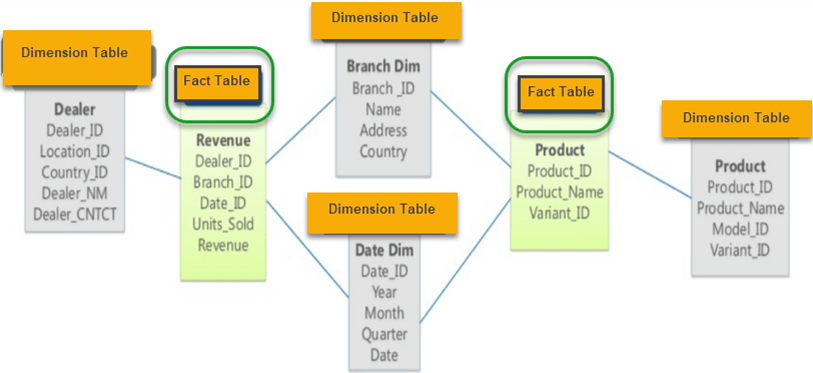
\includegraphics[scale=0.5]{images/Galaxy.png}
  \caption[Galaxy Schema (01.04.2020)]{Galaxy Schema (01.04.2020)}
  \label{fig:Galaxy-Schema}
  \url{https://www.guru99.com/images/1/022218_0758_StarandSnow3.png}
\end{figure}
\newpage
\subsection{OLAP Würfel}\label{ssec:Olap-Cube}
Im Star- beziehungsweise Snowflake Schema wird oft von Dimensionstabellen gesprochen, da sich jede Tabelle als eine Dimension eines OLAP Würfels darstellen lässt. Dies ermöglicht Analysten, die im Data Warehouse gespeicherten Fakten in Relation zu verschieden vielen Referenzinformationen zu setzen, um Kennzahlen wie den Umsatz anhand verschiedener Aspekte mehrdimensional zu analysieren und in diversen Detaillierungsstufen zu untersuchen.\\ 
Die nächste eingefügte Graphik \ref{fig:OLAP-Cube} zeigt die Darstellung eines dreidimensionalen OLAP Würfels, dessen Kanten verschiedene Dimensionen anzeigen. Die Länge wird durch die Anzahl der Zellen bestimmt. Jede einzelne Zelle des Würfels enthält genau einen Wert. Doch ist das OLAP Verfahren nicht auf drei Dimensionen beschränkt, sondern ist n-dimensional aufgebaut. Es ist möglich, beliebig viele Dimensionen zu umfassen.
\begin{figure}[H]
\centering
  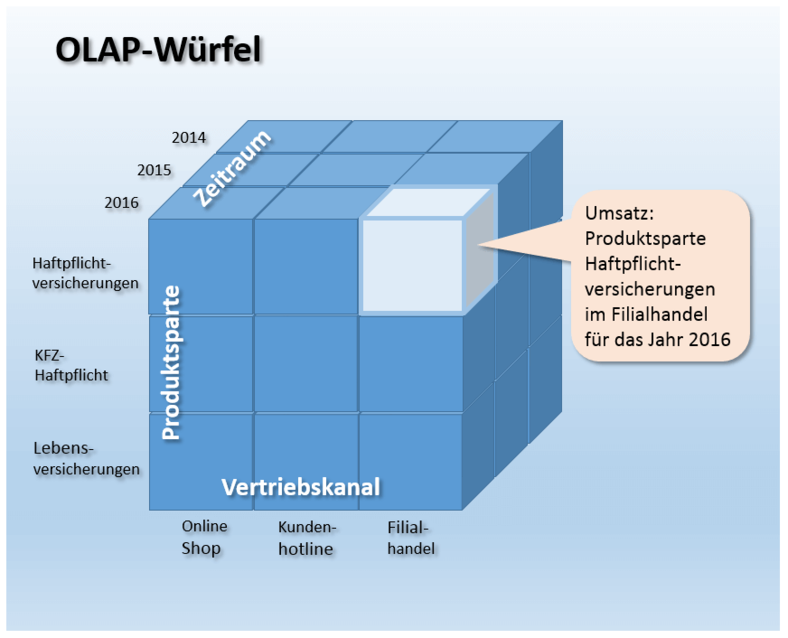
\includegraphics[scale=0.5]{images/OLAP.png}
  \caption[OLAP Cube (01.04.2020)]{OLAP Cube (01.04.2020)}
  \url{https://www.ionos.at/digitalguide/fileadmin/DigitalGuide/Screenshots/schematische-darstellung-eines-olap-wuerfels.png}
  \label{fig:OLAP-Cube}
\end{figure}
\newpage
\subsection{Datenbereitstellungsebene}
Diese Ebene ist die Schnittstelle zwischen Endanwendungen und Präsentationswerkzeugen. Methoden zur Auswertung und Analyse von Daten werden oftmals von diversen Endanwender Tools zur Verfügung gestellt. Diese Tools ermöglichen es, Informationen aus dem Bestand des Data Warehouses zu extrahieren und für den Endanwender in unterschiedlichen Darstellungsformen aufzubereiten. Das Spektrum umfasst Bericht- und Abfragewerkzeuge, \ref{ssec:Bericht-Werkzeug} Kollaborations Tools, \ref{ssec:Kollab-Werkzeug} Data Mining Tools, \ref{ssec:Data-Minging} Werkzeuge des OLAP \ref{ssec:Werkzeuge-OLAP}, und Forecasting- und Simulations Tools \ref{ssec:Forecasting-Tools}.
\subsection{Bericht- und Abfragewerkzeuge}\label{ssec:Bericht-Werkzeug}
Diese Tools ermöglichen es, Endanwender unterschiedliche Funktionen zu benutzen, um vordefinierte Standardberichte erstellen zu können. Diese Berichte können automatisch in einem regelmäßigen Abstand oder nach Abfrage erstellt werden. Um Benutzeranfragen an das Data Warehouse zu erleichtern, kann auf ein Anfrage Assistent Tool zurückgegriffen werden.
\subsection{Kollaborations Tools}\label{ssec:Kollab-Werkzeug}
Durch dieses Tool können die Kommunikation und Zusammenarbeit verschiedener Endbenutzer bei der Datenanalyse unterstützt werden. Einige der Funktionen sind das Speichern von Anmerkungen und der Austausch von Analyseergebnissen.
\subsection{Data Mining Tools}\label{ssec:Data-Minging}
Unter den Begriff Data Mining fallen alle ungerichteten als auch teilweise automatisierten Analysemethoden, die es darauf abgezielt haben, relevante Muster, Trends und Beziehungen im Datenbestand zu ermitteln. Data Mining Tools bauen auf statistische und mathematische Methoden, sowie Techniken aus der Künstlichen Intelligenz (KI) und des Maschinenlernens (ML) auf. Daten, die in Unternehmen für die Analyse eines Data Warehouse erzeugt und verarbeitet werden wachsen exponentiell. Da sich weltweit das durchschnittliche Datenvolumen alle zwei Jahre verdoppelt, gewinnen Data Mining Tools und Methoden im Rahmen des Data Warehousings immer mehr an Bedeutung.
\subsection{Werkzeuge des OLAP}\label{ssec:Werkzeuge-OLAP}
Von allen zur Verfügung stehenden Datenauswertungs- und Datenanalyse Tools haben sich im Rahmen des Datawarehousing vor allem OLAP Anwendungen als Standardbenutzerschnittstelle herauskristallisiert. Tools die im Rahmen des OLAP angewandt werden, stellen Endbenutzer verschiedenste Funktionen zur Verfügung. Mit diesen können Anfragen an das Data Warehouse ad-hoc formuliert werden. Sie dienen als Navigation durch den OLAP Würfel \ref{ssec:Olap-Cube}. 

Die Darstellung in so einem Würfel ermöglicht es, aufbereitete Daten in Abhängigkeit zu beliebig vielen vordefinierten Dimensionen zu modellieren. Um den OLAP Würfel richtig zu bearbeiten gibt es folgende Grundoperationen um dies zu ermöglichen.

\subsubsection{Slicing}\label{ssec:Slicing}
Diese Grundoperation kann eine Dimensionen eines OLAP Würfels auf eine Teilmenge begrenzen. Es wird ein Teil des gesamten Datenbestandes aus dem Datenwürfel herausgeschnitten und separat betrachtet.
\begin{figure}[H]
\centering
  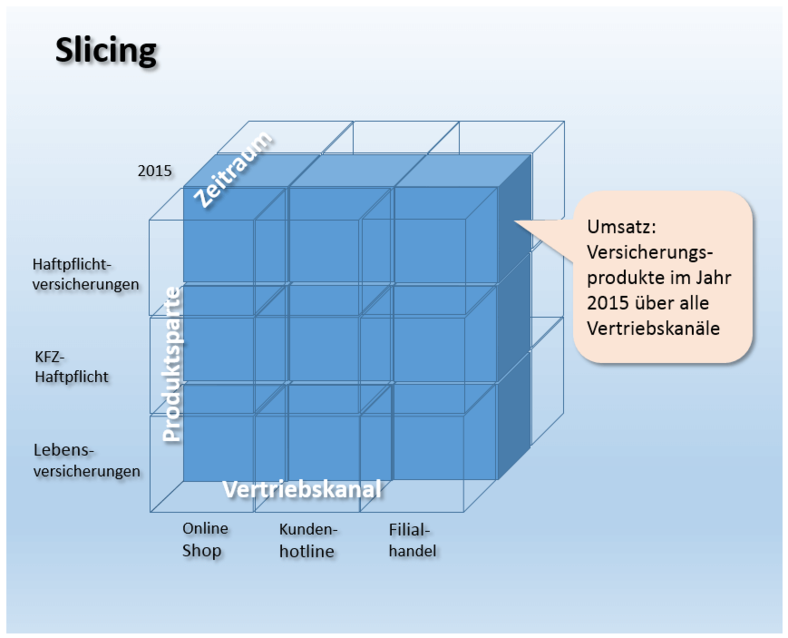
\includegraphics[scale=0.4]{images/Slicing.png}
  \caption[Slicing (01.04.2020)]{Slicing (01.04.2020)}
  {https://www.ionos.at/digitalguide/fileadmin/DigitalGuide/Screenshots/schematische-darstellung-einer-slicing-operation-am-beispiel-eines-dreidimensionalen-olap-wuerfels.png}
  \label{fig:Slicing}
\end{figure}
\newpage
\subsubsection{Dicing}\label{ssec:Dicing}
Wird ein OLAP Würfel durch mehrere Slicing \ref{ssec:Slicing} Operationen in verschiedenen Dimensionen beschnitten, spricht man von Dicing. Wenn Dicing durchgeführt wird, kommt ein kleinerer Würfel als Ergebnis heraus, der eine Teilmenge des Ganzen Würfels darstellt.
\begin{figure}[H]
\centering
  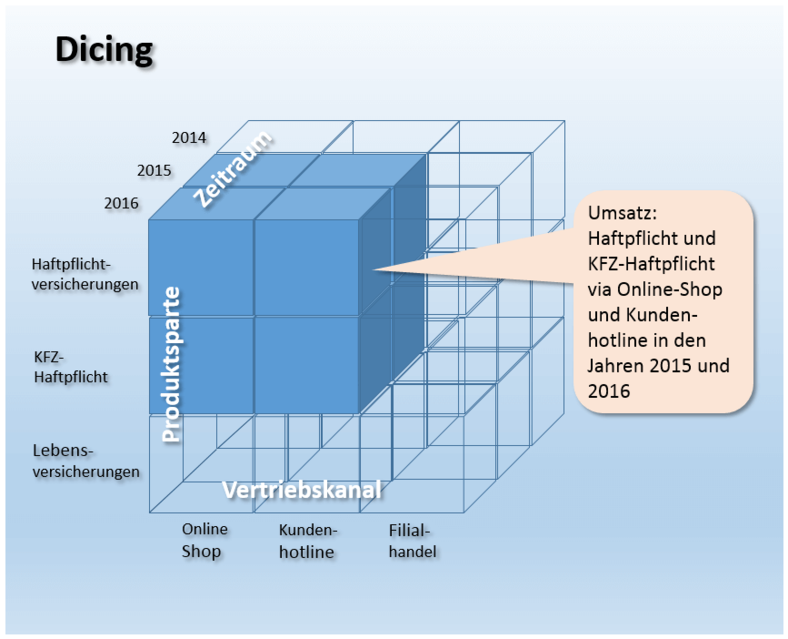
\includegraphics[scale=0.4]{images/Dicing.png}
  \caption[Dicing (01.04.2020)]{Dicing (01.04.2020)}
  {https://www.ionos.at/digitalguide/fileadmin/DigitalGuide/Screenshots/schematische-darstellung-einer-dicing-operation-am-beispiel-eines-dreidimensionalen-olap-wuerfel.png}
  \label{fig:Dicing}
\end{figure}
\newpage
\subsubsection{Pivoting}\label{ssec:Pivoting}
Pivoting ist das Drehen des Würfels. Wenn diese Funktion benutzt wird, wird eine andere Dimension des Gesamtwürfels sichtbar.
\begin{figure}[H]
\centering
  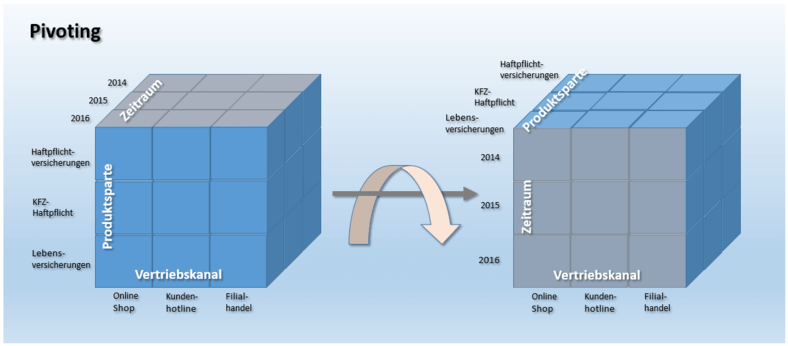
\includegraphics[scale=0.33]{images/Pivoting.png}
  \caption[Pivoting (01.04.2020)]{Pivoting (01.04.2020)}
  {https://www.ionos.at/digitalguide/fileadmin/DigitalGuide/Screenshots/schematische-darstellung-einer-pivoting-operation-am-beispiel-eines-dreidimensionalen-olap-wuerfel.png}
  \label{fig:Pivoting}
\end{figure}
\subsubsection{Drill Down / Roll Up}\label{ssec:Drill-Down}
Sollen die Aggregationen eines Objekts auf detaillierte Werte gebracht werden, kommt die Funktion Drill Down zum Einsatz. Diese Operation ermöglicht es Analysten in einem OLAP Würfel die Daten genauer darzustellen, um somit auch die Granularität der Daten zu erhöhen. Roll Up ist die Gegenoperation von Drill Down. Die Roll Up Funktion verdichtet die Informationen auf höhere Hierachiestufen. Diese beiden Operationen kommen zum Einsatz, um durch eine mehrdimensionale hierarchische Struktur hindurch zu navigieren.
\begin{figure}[H]
\centering
  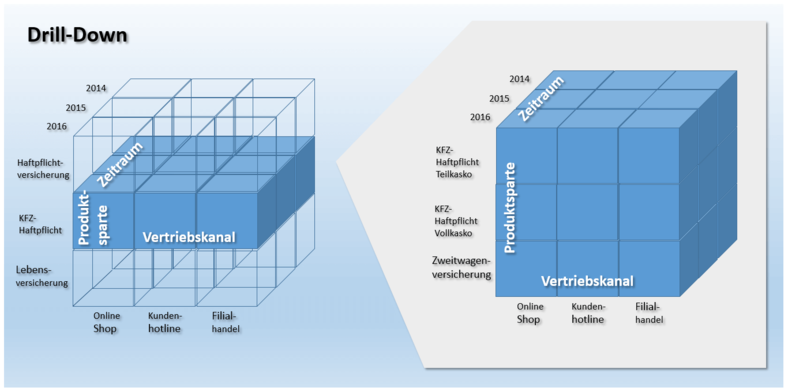
\includegraphics[scale=0.3]{images/Drill-Down.png}
  \caption[Drill Down]{Drill Down}
  {https://www.ionos.at/digitalguide/fileadmin/DigitalGuide/Screenshots/schematische-darstellung-einer-drill-down-operation-am-beispiel-eines-dreidimensionalen-olap-wuerfel.png}
  \label{fig:Drill-Down}
\end{figure}
\subsubsection{Drill Out / Split}\label{ssec:Drill-Out}
Drill Out ermöglicht es Benutzern, einem OLAP Würfel weitere Dimensionen hinzuzufügen. Das Ergebnis dieser Funktion sind detailliertere Daten. Doch anders als bei Drill Down wird der Grad nicht durch die Granularität gewonnen, sonder durch Informationsgewinn. Dieser Gewinn kommt durch die zusätzlichen Referenzinformationen der hinzugefügten Dimension zustande. Die Granularität bleibt erhalten.
\subsubsection{Drill In / Merge}\label{ssec:Drill-In}
Als Gegenoperation zu Drill Out \ref{ssec:Drill-Out} wird der Detailgrad des OLAP Würfels beim Drill In verringert. Dies passiert, indem eine Dimension entfernt wird. Im Gegensatz zu Roll Up kommt der Informationsverlust nicht aus der Veränderung der Betrachtungsebene, sonder durch den Verlust von dimensionaler Information. Auch hier bleibt die Granularität gleich. 
\subsubsection{Drill Across}\label{ssec:Drill-Across}
Diese Operation ermöglicht es auf mehreren OLAP Würfel, globale Analysen durchzuführen. Hier können beliebig viele Faktentabellen mit mindestens einer Dimension analysiert werden. Diese Dimensionen müssen aber die gleiche Hierachiestufe und Granularität aufweisen. 
\subsubsection{Drill Through}\label{ssec:Drill-Through}
In dieser Operation wird eine Zelle des Datenwürfels ausgewählt und im höchsten Detaillierungsgrad betrachtet. Anders als bei Drill Down wird bei Drill Through auf die Quelldaten der Würfelzelle zugegriffen. Das Resultat wird somit aus den Tabellenzellen abgeleitet, die der Berechnung der Würfelzelle zugrunde liegt.
\subsection{Forecasting und Simulations Tools}\label{ssec:Forecasting-Tools}
Diese Tools bieten Endanwendern die Möglichkeit, im Data Warehouse gespeicherte Kennzahlen in die Zukunft fortzuschreiben, um Vorhersagemodelle erstellen zu können. 
\newpage
\subsection{Data Warehouse Management}
In allen Ebenen des Data Warehouses sind spezielle Tools aktiv, die im Bereich Data Warehouse Management zusammengefasst werden. Aufgaben dieser Tools sind der Aufbau, die Wartung und der Betrieb aller Administrationsfunktionen, die im Rahmen des Data Warehousings benötigt werden. Zentrale Aufgaben des Data Warehouse Managements sind das Sicherheitsmanagement sowie das Systemmanagement.
\subsubsection{Scheduling}\label{ssec:Scheduling}
Das Scheduling umfasst die Steuerung der Data Warehouse Prozesse. Administrationsfunktionen im Rahmen des Schedulings lassen sich in Bezug auf die Ebene der Data Warehouse Architektur kategorisieren.
\subsubsection{Datenerfassung / Datenintegration}\label{ssec:Datenerfassung}
Auf der Datenerfassungsebene ist der Data Warehouse Manager für das Design und die Anpassung des ETL-Prozess zuständig. Darüber hinaus werden diese Funktionen bereitgestellt, um Aktualisierungsvorgänge und das Qualitätsmanagement zu überwachen.
\subsubsection{Datenhaltung}\label{ssec:Datenhaltung}
In der Datenhaltung überwachet der Data Warehouse Manager, die Speicherauslastung, konstruiert Aggregationstabellen und führt Archievierungsoperationen und Backupoperationen durch.
\subsubsection{Datenbereitstellung}\label{ssec:Datenbereitstellung}
Administrationsfunktionen auf dieser Ebene umfassen die Benutzerverwaltung als auch die Überwachung von Anfragelaufzeiten. 
\subsubsection{Metadaten Management}\label{ssec:Metadaten-Management}
Die zentrale Komponente des Data Warehouse Managers ist das Metadaten Repository. Dieses enthält alle Informationen, die für die Konstruktionen und den Betrieb des Data Warehouses erforderlich sind, sowie Informationen über den Datenbestand. Im Repository  gespeicherte Metadaten umfassen die Definition des zugrundeliegenden Datenbank Shemas, Informationen zu Speicherstrukturen, Zugriffspfade und Dateigrößen, Metdaten zur Beschreibung der Datenquellen. Auch sind Aktualisierungszeitpunkte, Datenbereinigungs- und Transformationsregeln, Indizes und Partitionstabellen dort hinterlegt. Darüber hinaus sorgt der Data Warehouse Manager für einen Austausch der Metadaten zwischen den einzelnen Komponenten des Data Warehouses. So wird eine homogene Metadatenbasis bereitgestellt.
\subsubsection{Sicherheitsmanagement}\label{ssec:Sicherheitsmanagement}
Das Sicherheitsmanagement umfasst diverse Dienste im Rahmen der Nutzerauthentifizierung. Auch wird die Autorisierung und Verschlüsselung berücksichtigt.
\subsubsection{Systemanagement}\label{ssec:Systemmanagement}
Im Rahmen des Systemmangements stellt der Data Warehouse Manager verschiedene Funktionen für den Betrieb des Data Warehouses bereit. Diese umfassen das Monitoring, die Datenarchivierung oder die Datensicherung.